% THIS IS SIGPROC-SP.TEX - VERSION 3.1
% WORKS WITH V3.2SP OF ACM_PROC_ARTICLE-SP.CLS
% APRIL 2009
%
% It is an example file showing how to use the 'acm_proc_article-sp.cls' V3.2SP
% LaTeX2e document class file for Conference Proceedings submissions.
% ----------------------------------------------------------------------------------------------------------------
% This .tex file (and associated .cls V3.2SP) *DOES NOT* produce:
%       1) The Permission Statement
%       2) The Conference (location) Info information
%       3) The Copyright Line with ACM data
%       4) Page numbering
% ---------------------------------------------------------------------------------------------------------------
% It is an example which *does* use the .bib file (from which the .bbl file
% is produced).
% REMEMBER HOWEVER: After having produced the .bbl file,
% and prior to final submission,
% you need to 'insert'  your .bbl file into your source .tex file so as to provide
% ONE 'self-contained' source file.
%
% Questions regarding SIGS should be sent to
% Adrienne Griscti ---> griscti@acm.org
%
% Questions/suggestions regarding the guidelines, .tex and .cls files, etc. to
% Gerald Murray ---> murray@hq.acm.org
%
% For tracking purposes - this is V3.1SP - APRIL 2009

\documentclass{acm_proc_article-sp}
\usepackage{balance}  % to better equalize the last page
\usepackage{graphics} % for EPS, load graphicx instead
\usepackage{times}    % comment if you want LaTeX's default font
\usepackage{url}      % llt: nicely formatted URLs
\usepackage{multicol}% http://ctan.org/pkg/multicols
\usepackage{graphicx}% http://ctan.org/pkg/graphicx
\usepackage{float}
\usepackage{capt-of}

\begin{document}

\title{Glass Shooter: Exploring First-Person Shooter\\ Game Control with Google Glass}

\numberofauthors{1} 
\author{\alignauthor Chun-Yen Hsu, Ying-Chao Tung, Silvia Chyou, \\Han-Yu Wang, Jer-Wei Lin, Mike Y. Chen\\
\affaddr{Mobile and HCI Research Lab, National Taiwan University} \\ 
\email{\{hcythomas0125,tony61507,silvia.chyou,huw12313212,evin92\}@gmail.com,\\ mikechen@csie.ntu.edu.tw}
}



\makeatletter
\def\url@leostyle{%
  \@ifundefined{selectfont}{\def\UrlFont{\sf}}{\def\UrlFont{\small\bf\ttfamily}}}
\makeatother
\urlstyle{leo}
\makeatletter
\let\@oldmaketitle\@maketitle% Store \@maketitle
\renewcommand{\@maketitle}{\@oldmaketitle% Update \@maketitle to insert...
  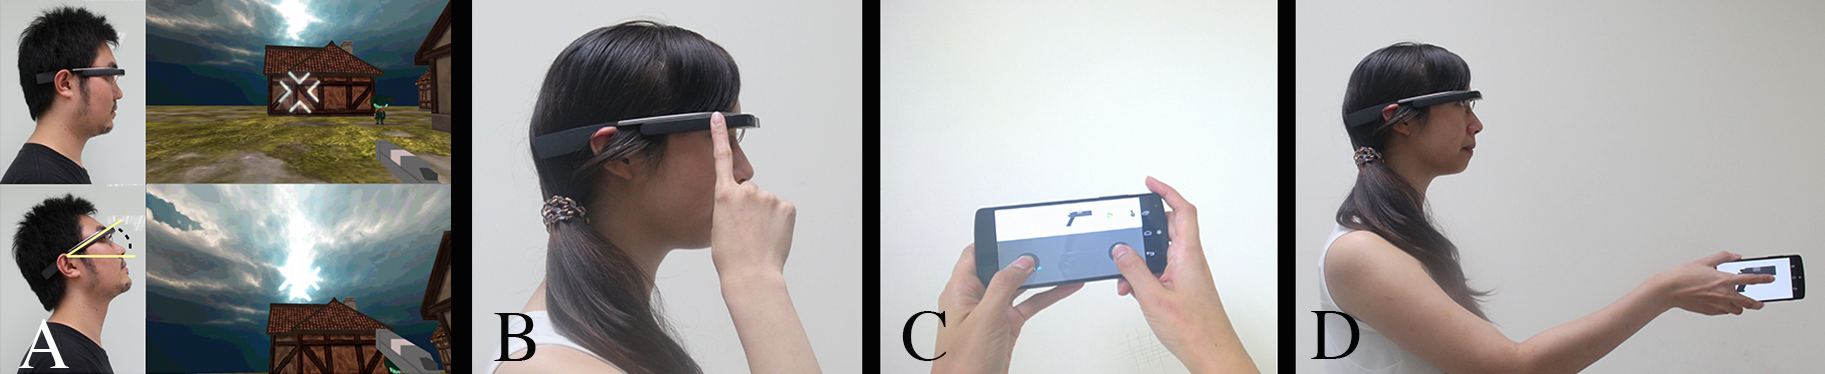
\includegraphics[width=1\linewidth]
    {GlassGame2.png}
       \captionof{figure}{We implement multiple possible control methods for ``Glass Shooter''. (A) Our demos uses head mounted gyroscope to control the first-person viewport. (B) We designed a set of gestures on the touchpad strip: Players can move forward by touching the front half of the touchpad, and move backward by touching the rear half. Weapons can be fired by using taps. (C) Smartphones as virtual controller: two virtual joysticks and buttons to move and to change the viewport and to fire weapons; (D) Considering smart phone as a small gun: the player can use her phone orientation to aim the target.}
  \label{fig:figure}\bigskip
    }% ... an image

\makeatother

\maketitle
\begin{abstract}
Smart Glasses offer the opportunity to use head mounted sensors, such as gyroscope and accelerometers, to enable new types of game interaction. To better understand game play experience on Smart Glasses, we recruited 24 participants to play four current games on Google Glass that uses different interaction methods, including gyroscope, voice, touchpad, and in-air gesture. Study results showed that participants were concerned with comfort and social acceptance. Also, their favorite input method was gyroscope, and their favorite game type was First-Person Shooter (FPS) game. Hence, we implemented a FPS game on Google Glass using gyroscope for changing the viewport(see Figure~\ref{fig:figure}.A), and divide FPS controls into four categories: (a)Viewport Control, (b)Aim Control, (c)Fire Control, (d)Move Control. We implemented multiple control methods in each category to evaluate and explore glass game control design.
\end{abstract}


\category{K.8.0.}{Personal Computing}{General Games}

\terms{Human Factors}

\keywords{Google Glass, Wearable Devices, Game Design, Head Mounted Display, Multi-Modal, Mobile Phone, Gestures. }

\section{Introduction}
%Games are the most popular type of mobile apps, with recent statistics showing that 70-80\% of all mobile downloads being mobile games\cite{statistics,infographic}. Although traditional game design has many well-known guidelines~\cite{videogame,mobilegame,bodygame,gameflow,argame,wearable}, game design for Smart Glasses has not been explored.% computers are claimed to be the next evolution beyond smartphones. 
%Game is one of the most important application in computer science.

%There are several Smart Glasses products on the market over these years, we choose the most famous one, Google Glass, as our main research platform. To realize the current gameplay experience on google glass, 
Smart Glasses provide several new features, such as always available display, head mounted sensors, and first-person viewport. These new elements do not exist in the traditional game platform. How to apply these techniques to create a relevant game experience on Smart Glasses is still an unexplored area.

To better understand game design for Smart Glasses, we invited 24 users to play 4 existing games~\cite{minigame} on the most popular Smart Glasses, Google Glass. The four games have been selected to span different game types and control styles. Our study showed three design challenges that are not discussed in current game design guidelines: ``Limited control'', ``Eye strain'' and ``Social acceptance''. Moreover, after playing these 4 selected glass games, most participants expressed that they prefer to play First-Person Shooter(FPS) game on Google Glass. 

%Also, compared with other gaming platforms, Smart Glasses lack traditional input method like mouse, keyboard, joystick, or touch screen. However, there are some non-traditional wearable sensors such as camera, touchpad, microphone, gyroscope, and accelerometer. Our study showed that most of the users preferred using gyro, and preferred playing First-Person Shooter (FPS) games on Google Glass. Therefore, we implement a FPS game,``Glass Shooter'', with multiple control styles to explore game design space for Smart Glasses and to understand user preference.
%This demo focuses on exploring the ``limited control'' issue and compares Glass-only input to Glass+smartphone input. 

In this demo, we focus on the issue ``Limited control''. Compared with other gaming platforms, Smart Glasses lack traditional input method like mouse, keyboard, joystick, or touch screen. However, there are some non-traditional wearable sensors such as camera, touchpad, microphone, gyroscope, and accelerometer.  

%Eyewear computers, such as google glasses implementation, are claimed to be the next evolution beyond smartphones. In addition, game industry in the US earned about 21.53 dollars in 2014\cite{essentialfacts}. Recent statistics show that around 70-80\% of all mobile downloads is composed of mobile games\cite{statistics,infographic}. Traditional game design has tons of guidelines\cite{videogame,mobilegame,bodygame,gameflow,argame,wearable}. However, the game design for smart glass game is still an unexplored area. Hence, we want to explore the game design space on smart glass. And after concerning current market share, we choose Google Glass as our candidate.

%First we want to realize the current game play experience on google glass, so we recruited 24 users to play existing google glass game\cite{minigame} with different content or control style. After user study, we found that about one third of users want to play First-Person Shooter(FPS) game on google glass. So we decide to implement a FPS game on google glass for demonstration. In addition, we also provide multiple control styles to evaluate and find out the best control way on google glass. 

%\section{Game Prototype}


Considering traditional game design and new features on Smart Glasses, we implement a game, ``Glass Shooter'', a FPS game with multiple control styles on Google Glass. With ``Glass Shooter'', we can collect user feedback of different control schemes and understand user preference. 
%so that we can have some control variable to change directly by ourselves and compare with different settings. 
%According to user imagination from user study 1, there are five different type of game which players suggest. We choose FPS, with the highest number of users who wants to play, as our game type.
%And FPS also has the most control issues in it's type. 
%We expect that our FPS game can satisfy most user and get useful knowledge by studying and implement this type of game.

\section{Control}
There are four main controls in FPS games: (a)Viewport Control, (b)Aim Control, (c)Fire Control, (d)Move Control.
With Viewport Control, users can change camera's perspective and observe the surrounding environment.
Aim Control is about how players moving the crosshair.
%The third control is fire control, laying stress on how player trigger the fire to beat their enemy. 
%And the last one is the move control, which focuses on how  player controls avator's position and dodges the bullet from enemy.
Besides, users open fire with Fire Control and move their avators through Move Control in the game.

%Although smart glass is new wearable device to interact with users and will be more powerful in the future, it does not meant that smart glass will replace smart phone\cite{lecture}. 
%With these two different typies of device, they should complement each other to make up their own deficiency.
%Furthermore, google glass is designed to always connects with smart phone through bluetooth. So we can include smart phone as controller for our game designs and control scheme intuitively.
To extend the diversity of our input controls, we design control methods not only with input manners available on Google Glass, but also with possible game control methods on Smart Phones.

According to previous work\cite{headvideo,tele,robot,viewport}, using head orientation as a Viewport Control is undoubtedly intuitive.%However, we can't confirm whether using head orientation is really suitable for users to aim the target.
Therefore, in this work, we only explore the remaining control problems on Aim Control, Fire Control, and Move Control. 
First, we supposed 3 different aim control schemes to test which would be the most favorite control for users. 
Three different Aim Control schemes are listing below:

\begin{enumerate}
\item Viewport aiming scheme: The crosshair is always at the center of the viewport. Player can aim the enemy by using their head to move their viewport. In other words, player are using head orientation to aim the target.

\item Gun aiming scheme: Considering your smart phone as a small gun. The player can use the phone orientation to aim the target. The crosshair will be controlled by the direction of the phone.(see Figure~\ref{fig:figure}.D)

\item Phone joystick scheme: Using smart phone as a joystick to move the crosshair on the glass screen.(see Figure~\ref{fig:figure}.C)
\end{enumerate}

We also bring up 3 different fire controls as below:

\begin{enumerate}
\item Phone trigger scheme: Using touch screen on mobile phone as the fire trigger. Players can just open fire by tapping their phone touchscreen.

\item Glass tapping scheme: Player uses fingers to tap on glass touchpad to open fire.(see Figure~\ref{fig:figure}.B)

\item Voice control scheme: Player uses voice control, such as the sound of ``Bang'', to open fire.

\item Eye winking scheme: Player uses intentional eye winking as a fire trigger.
\end{enumerate}

We propose 4 moving control schemes:

\begin{enumerate}
\item Head gesture scheme: We implement the system from the work of Hinkel et al.\cite{wheel} in our FPS game control system.

\item Glass touchpad: We designed a set of gestures on the touchpad strip. Players can move forward by touching the front half of the touchpad, and move backward by touching the rear half.

\item Phone controller scheme: Using virtual joystick on Smart Phone to move the character.

\item On track moving scheme: There exists possibilities that controlling player's movement is not completely suitable for glass game. Therefore, we design a pre-defined track for player in this scheme, and the avatar will move on the track automaticlly. So player can focus on aiming and fighting, rather than the movement control.
\end{enumerate}
%\subsubsection{Phone aiming}
% Aiming by using smart phone as a gun
%By using both of our hands, we can hold the smart phone with the same posture as we hold a gun. With this pose, we can switch our angle of view by revolving our body. And by using gyro, we can aim the target or the enemy by trimming our smart phone to shoot precisely. In other words, we can use smart phone as a aiming device, such as players using an electric torch or a gun.

%\subsubsection{Thrower}
% Using smart phone as body motion sensing
%Take Nintendo Wii for example, players movement can be detected precisely by the sensor. Although google glass can't have as strong sensor as Nintendo Wii, we still can detect some players' movement by our controller, smar phone. For instance, players hold the smart phone and can do throwing motion to simulate as throwing the hand grenade, and can make waving motion as waving the knife, and so on.

%\subsubsection{Driving simulation}
%While player driving the car, player use controller to emulate their motion as driving the car. It can indead raise players' game play experience greatly. So we can hold our controller, smart phone, as a steering wheel by both user's hand, and revolving the smart phone to emulate turning of the steering wheel.

%\subsubsection{Traditional joystick}
%To compare various of control method, we also provide traditional joystick for players on our controller, smart phone. By using traditional joystick, players can turning their angle of view and move their position directily.

\section{Conclusion and Future Work}
We have invited 24 players to play 4 different built-in games on google glass. Through the investigations, we observed three main categories of challenges we may meet when developing glass games, which are ``Limited control'', ``Eye strain'' and ``Social acceptance'' respectively. And we cast our focus mainly on discussing ``limited control'', about different types of controlling methods we may encounter in a first-person shooter game on glasses.
Therefore, after refering to both previous game design and glass features, we've classified the control issues among FPS glass game into four main categories as follows: viewport control, aimimg control, firing control, and last but not least, the moving control. For all these four terms of controls mentioned above, we've proposed several methods to meet the requirements seperately.
In the future, we will conduct a series of user studies to clarify which method is the most suitable for each four class of controls. Therefore we can develop a more intuitive controlling methods for FPS glass games. Furthermore, we will also move on to discuss the ``Eye Strain'' and ``Social Acceptance'' problems we brought up before.
%In this demonstration, we presented a first-person shooter game based on our user feedback from existing glass games. To explore the glass gaming control, which is still an open question nowadays, we designed and implemented multiple control styles; (a) Glass Control; (b) Smartphone as controllers; (c) Smartphone as tangible device; this work still lacks of system validation, so we are planning to perform a formal user study currently. Moreover, we are interested in ``Eye Strain'' and ``Social Acceptance'' problems on Google Glass because these puzzles do not appear in earlier works about other mobile devices.
%To explore the complete game design space on Google Glass, we will accomplish a series of user studies to evaluate these two issues we found in our previous study in the following months. 
%we hope our effort can inspire more glass game developers to develope more intuitive and suitable controls. With better gaming controls, we belive it can enhance glass game play experience significantly than before, and we also hope to be able to inspire more exploration of smart glasses gaming and spread game entertainment for more people.


\section{Acknowledgements}
We thank our advisor Prof. Mike Y. Chen and the faculty and staff of National Taiwan University. We should also like to express our gratitude towards all players and testers who have helped us in our many (buggy) iterations.


% That's all folks!
\bibliographystyle{abbrv}
\bibliography{sigproc}

\balancecolumns
\end{document}

